\documentclass[12pt]{article}
\usepackage{light}
\usepackage{enumerate}

\hidesolutions
%\showsolutions

\newcommand{\edge}[2]{#1\text{---}#2}
\newcommand{\mfigure}[3]{\bigskip\centerline{\resizebox{#1}{#2}{\includegraphics{#3}}}\bigskip}

\begin{document}

\recitation{12}{October 19, 2012}

%%%%%%%%%%%%%%%%%%%%%%%%%%%%%%%%%%%%%%%%%%%%%%%%%%%%%%%%%%%%%%%%%%%%%%%%%%%%%%%

\newcommand{\bigbox}{\fbox{\vspace{0.5in} \hspace{0.75in}}}

\section{The L-tower problem}

%% Prof Leighton suggests the following changes: as part of the question, we should ask them to figure out what the condition on x is for near instabiility. We can also ask for a condition on x for when it is most stable. The latter is when x is close to an even integer. 

Observe the structures shown in Figure~\ref{fig:towers}.  One has 2 L-shapes, the other 5 L-shapes. Consider a tower with $k$ L-shapes.  Assume that the blocks are all of size $x\times 1$ where $x > 1$. As the picture indicates,  if $k$ is too small then the tower falls to the left. On the other hand, if $k$ is too large the tower would fall to the right. Will the tower be stable for some $k$?  Prove there is at least one value of $k$ for which the L-tower is stable.  Assume that a structure is stable if and only if its center of gravity is not hanging in the air horizontally. The L-tower is stable if and only if each of its subparts is stable.   \\

\emph{Hint:}  Show the tower is stable if and only if $\frac{3x - 3}{2} \leq  k \leq \frac{3x - 1}{2} $.

\begin{figure}[h]

\centering
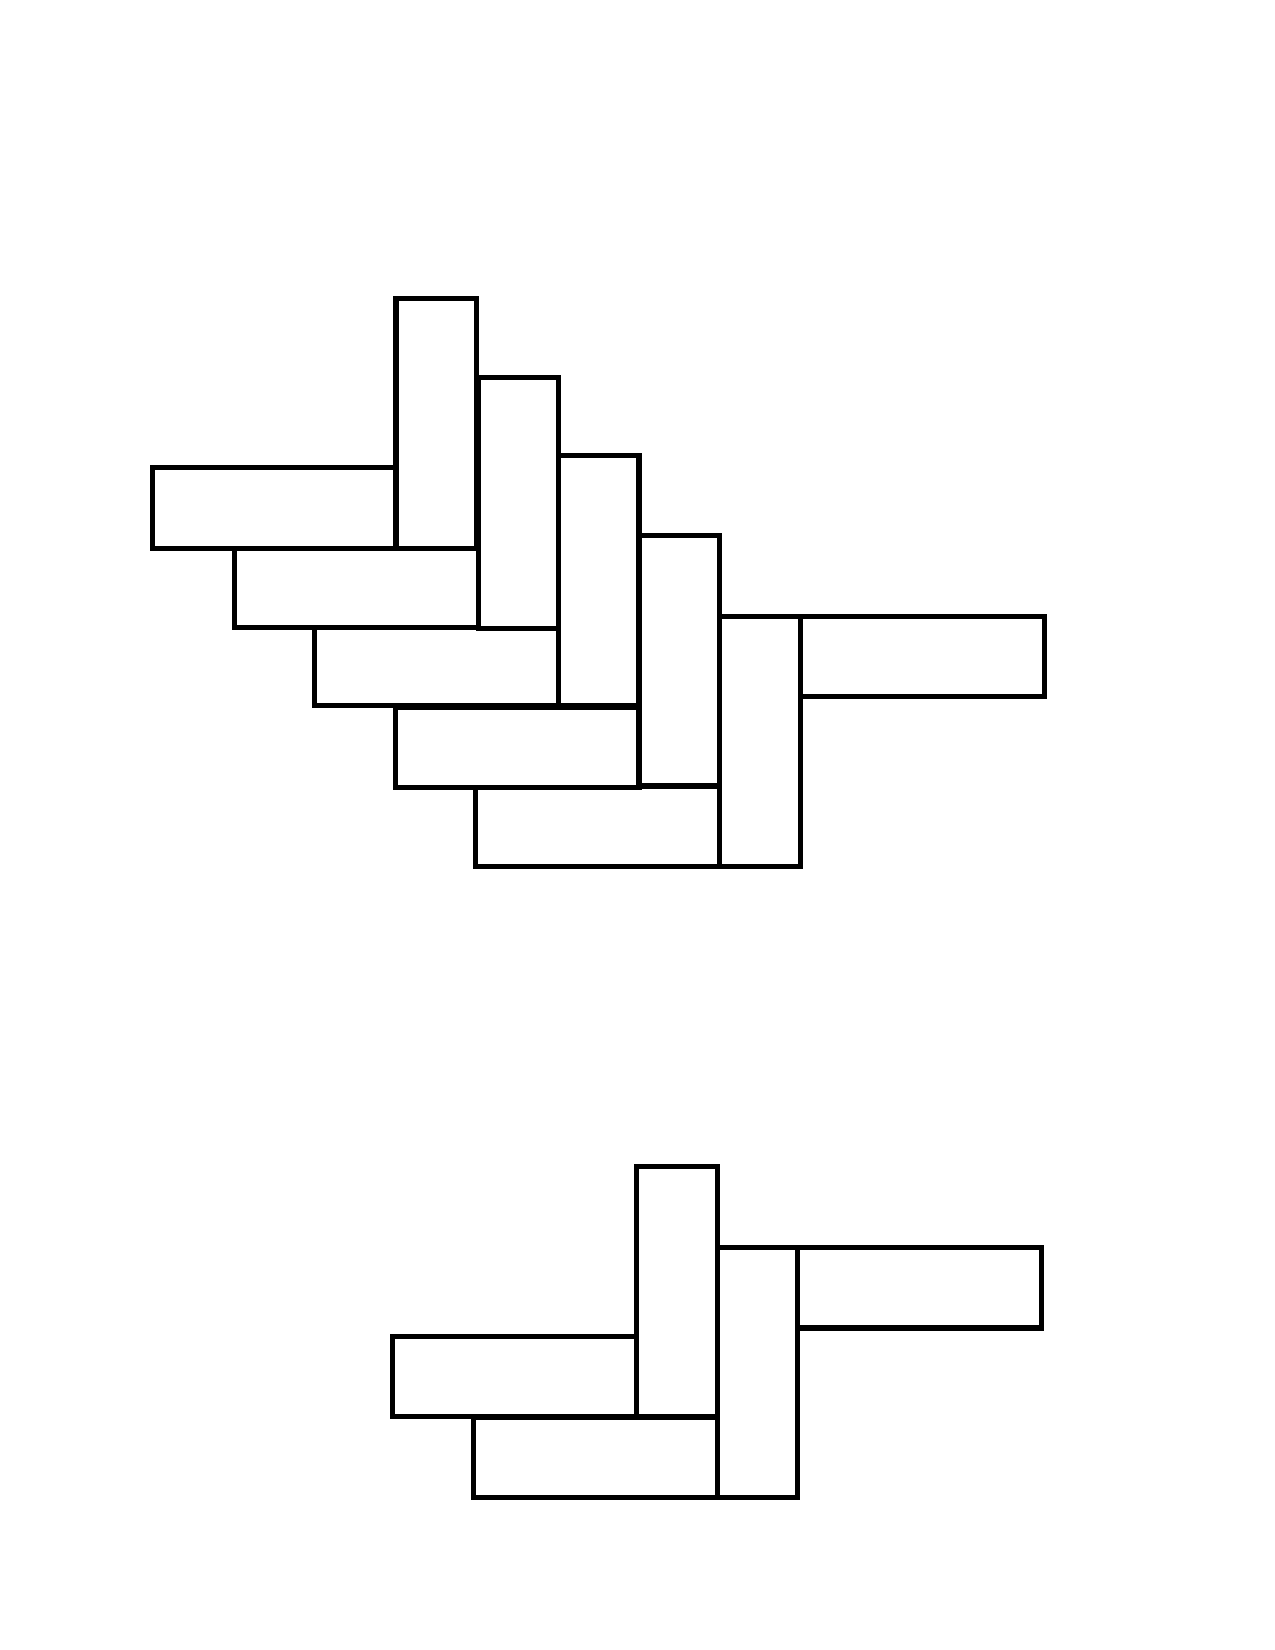
\includegraphics[scale=0.4, angle=-90]{Diagram1}
\caption{Too few or too many L shapes make the tower unstable \label{fig:towers}}
\end{figure}

\solution{
As indicated in the description, an arbitrary structure is considered stable if and only if its center of gravity lies on top of some form of support. For our L-towers this implies several conditions that must hold simultaneously. Consider the case $k=3$, illustrated in Figure~\ref{fig:conditions}. For the structure to be stable, we need the topmost L-shape to be stable on top of the second L-shape.  This is Condition 1.  We also need the structure formed by the topmost 2 L-shapes to be overall stable on top of the lowest L-shape. This is Condition 2. And finally, we need the three L-shapes to be stable on top of the single standing block. Call this Condition 3. In general, if there are $k$ L-shapes, there are $k$ conditions that must be satisfied for the structure to be stable. We will explicitly describe these constraints below.

\begin{figure}
\centering
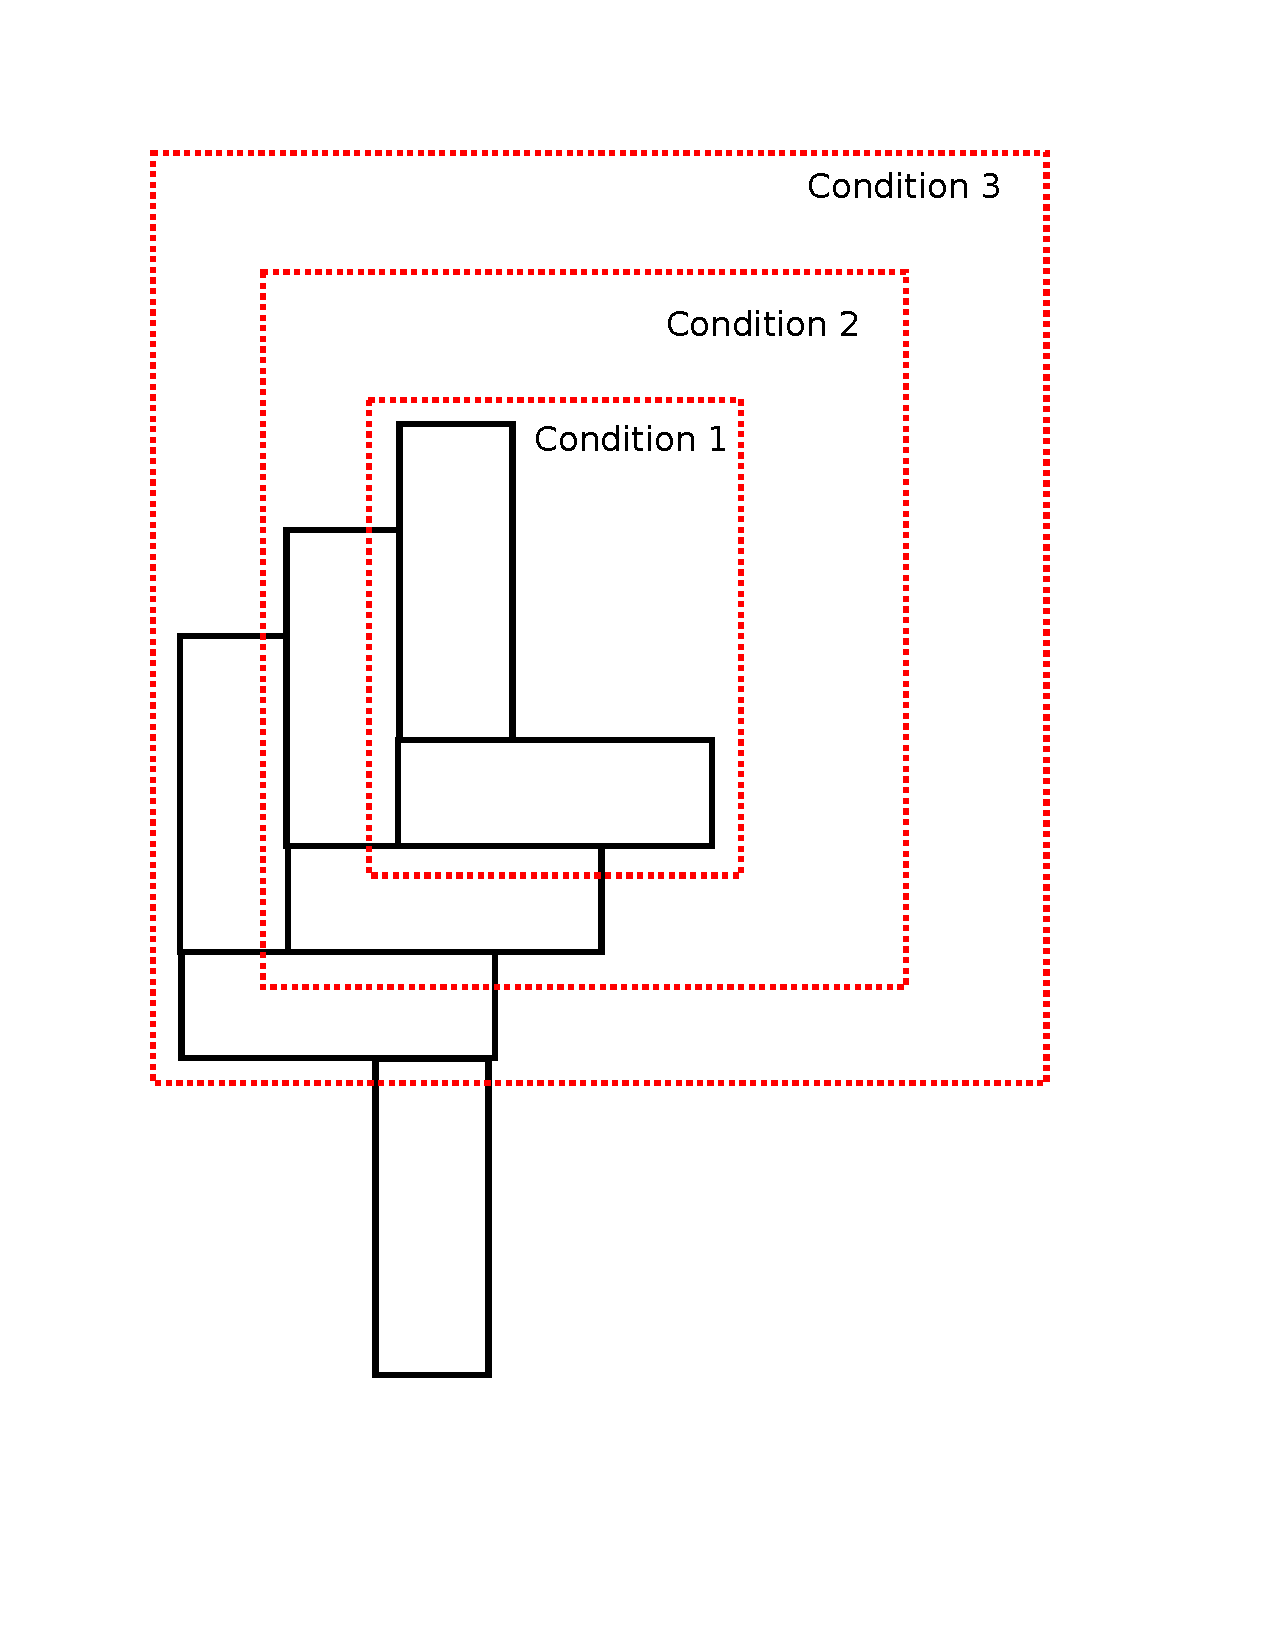
\includegraphics[scale = 0.4]{sol1}
\caption{Three necessary conditions for stability, when $k = 3$ \label{fig:conditions}. Put together, we also consider them sufficient.}
\end{figure}

Throughout the solution we are only concerned with the x-coordinates of the center of mass. The center of mass of a set of L-shapes can be computed by partitioning the figure into individual L shapes, and then averaging their individual centers. 

Let $c_1$ be the position of the center of mass for an individual L-shape starts at $0$. The vertical block has its center at $1/2$, the horizontal block at $x/2$. Hence, the center of a single L-shape is $(1/2 + x/2)/2 = (x + 1)/4$ to the right of where it starts.

Now let $c_h$ be the position for the center of mass of $h$ L-shapes stacked together, where we have shifted our reference frame so that the structure starts at $0$. This new center of mass can be obtained from averaging the center of a single L shaped shifted by 1 every time. So we get $c_h = \left[ c_1 + (c_1 + 1) + \cdots + (c_1 + (h -1))\right] / h$.  Regrouping, we get $c_h  = \left[ hc_1 + (1 + 2 + \cdots + (h-1)) \right] / h = \left[ hc_1 + h(h-1)/ 2 \right] /  h$, from where we arrive to: $c_h = c_1 + (h-1)/2$. 
It is helpful to think visually about this equation. When $h=1$, we naturally get $c_h = c_1$. As $h$ increases, the center shifts by $1/2$ to the right every time.

Now we can write explicitly all the conditions for a structure  with $k$ L-shapes to be stable. We need every structure to stand stable on top of the next L. If we imagine we have a stack of $i$ L-shapes starting at 0 on top of another L-shape starting at $-1$, we require:

$$c_i \leq x - 1$$

This simply means that if we have a stack of $i$ L-shapes starting right on the origin, we need its center of gravity to fall within the next L. The next L ends at $x-1$.

If we have $k$ L-shapes, this constraint applies to the first $k-1$ stacks. So we get the conditions:

$$c_1 \leq x-1$$
$$c_2 \leq x-1$$
$$\vdots$$
$$c_{k-1} \leq x-1$$

Finally, the overall stack of $k$ L-shapes has a slightly different requirement, since it stands on top of the vertical block:

$$x - 1 \leq  c_{k} \leq x$$

Now we need to find whether some $k$ satisfies all of these constraints. Recall $c_{k-1} > c_{k-2} > \cdots > c_{1}$, so we only need to check the last two constraints $c_{k-1} \leq x -1$ and $x - 1 \leq  c_{k} \leq x$. Substituting $c_k = (x+1)/4  + (k - 1)/2$ and $c_{k-1} = c_{k} - 1/2 = (x + 1)/4 + (k-1)/2 - 1/2$, we get the inequalities:

$$(x + 1)/4 + (k-1)/2 \leq  x - 1/2$$
$$ x - 1 \leq (x+1)/4 + (k-1)/2 \leq x$$

The first inequality is stronger on the right than the second, so consolidating both we get:

$$ x - 1 \leq  (x+1)/4 + (k-1)/2 \leq x - 1/2$$ which solved for $k$ yields:

$$\dfrac{3x - 3}{2} \leq k \leq \dfrac{3x- 1}{2}$$

There is a gap between the upper and lower bound of exactly 1. Hence either there is an integer right between them, or both are integers. For $(3x-3)/2$ to be an integer we need $x$ to be an odd integer.  Hence in the case where $x$ is an odd integer we have two choices of $k$ but on each the structure will be barely stable.

}
%%%%%%%%%%%%%%%%%%%%%%%%%%%%%%%%%%%%%%%%%%%%%%%%%%%%%%%%%%%%%%%%%%%%%%%%%%%%%%%
\newpage

\section{Double Sums}

Sometimes we have to evaluate sums of sums, otherwise known as
\emph{double summations}. It's good to know how to tame these beasts!
Here's an example of a double summation:
\[
\sum_{i=1}^n \sum_{j=1}^i j
\]
It looks ferocious...all those sharp teeth! But actually, this double
summation is just a sheep in wolf's clothing: to evaluate it, we can
just evaluate the inner sum, replace it with a closed form we already
know, and then evaluate the outer sum which no longer has a summation
inside it.

\begin{enumerate}[(a)]
\item Evaluate the summation. (\textit{Hint: $\sum(a+b)=\sum a + \sum b$.})

\solution[\vspace{3in}]{
\begin{align*}
\sum_{i=1}^n \sum_{j=1}^i j &= \sum_{i=1}^n \frac{i(i+1)}{2}\\
&= 1/2 \sum_{i=1}^n (i^2 + i)\\
&= 1/2(\sum_{i=1}^n i^2 + \sum_{i=1}^n i)\\
&= 1/2(\frac{n^3}{3} + \frac{n^2}{2} + \frac{n}{6} + \frac{n(n+1)}{2})\\
&= 1/2(\frac{n^3+3n^2+2n}{3})
\end{align*}
}
\end{enumerate}

Unfortunately, not all summations are so docile. Fortunately, we have
ways to deal with this. There's a special trick that is often
extremely useful for sums, and that is to \emph{exchange the order of
  summation.}  
%We'll go through an example here.


        Our goal will be to compute the following sum, for $n$ a positive integer:
        \[ S_n = \sum_{k=1}^n k2^k. \]
    There are various ways to handle it, but here we'll see a way that (surprisingly!) involves double sums. You may object that there is only a single sum. But here's a trick: we can rewrite $S_n$ as
    \[ S_n = \sum_{k=1}^n \sum_{j=1}^k 2^k. \]

    \begin{enumerate}[(a)]
        \setcounter{enumi}{1}

    \item 
    If we think about the
  pairs $(k,j)$ over which we are summing, they form a triangle in the
  table below. The values in the cells of the table correspond to the
  terms in the double summation. Complete this table to see the pattern.

\[
\begin{array}{c|cccccc}
    k\; {\setminus} \;j &1&2&3&4&\dots&n\\
\hline
1& \\
2 &\\
3 \\
4 \\
 &\dots\\
n &&&&&\dots
\end{array}
\]

\solution{
\[
\begin{array}{c|cccccc}
j&1&2&3&4&\dots&n\\
\hline
k\\
1&2\\
2 &4&4\\
3 & 8 & 8 & 8\\
4 & 16 & 16 & 16 & 16\\
 &\dots\\
n &2^n & 2^n & 2^n & 2^n &\dots& 2^n
\end{array}
\]
}

\item The summation above is summing each row and then adding the row
  sums.  But we can tame this beast if, instead, we first sum the
  columns and then add the column sums. Use the table to rewrite the
  double summation. The inner summation should sum over $k$, and the
  outer summation should sum over $j$.

\solution[\vspace{.5in}]{
\[ 
    S_n = \sum_{j=1}^n \sum_{k=j}^n 2^k.
\]
}

\item Now simplify the summation to derive a closed formula for $S_n$.

\solution[\vspace{3in}]{
    Recall the geometric sum formula $\sum_{k=0}^n 2^k = 2^{n+1} - 1$. From this (or directly) we obtain
    \[ \sum_{k=j}^n 2^k = 2^{n+1} - 2^{j}. \]
    Thus

\begin{align*}
    \sum_{j=1}^n \sum_{k=j}^n &= \sum_{j=1}^n (2^{n+1} - 2^j)\\
                              &= \sum_{j=1}^n 2^{n+1} - \sum_{j=1}^n 2^j\\
                              &= n \cdot 2^{n+1} - (2^{n+1} - 2^1)\\
                              &= (n-1)\cdot 2^{n+1} + 2.
\end{align*}
}

\end{enumerate}

Now try your hand at another double sum.

\begin{enumerate}[(a)]
        \setcounter{enumi}{4}

    \item 
    Find a formula for $F_n$, for $n$ a positive integer: % (your solution to the previous part might come in handy at some point...)
\[ F_n = \sum_{k=1}^n k \sum_{j=k}^n  2^j/(j+1). \]

 \solution{
     Exchanging the order of sums (you will probably want to draw a table as above to make sure you get the limits right), we obtain
 \begin{align*}
     F_n &= \sum_{j=1}^n \frac{2^j}{j+1} \sum_{k=1}^j k\\
         &= \sum_{j=1}^{n} \frac{2^j}{j+1} \cdot \frac{j(j+1)}{2}\\
     &= \tfrac12\sum_{j=1}^n j2^j\\
     &= \tfrac12S_n\\
     &= (n-1)2^n + 1.
 \end{align*}
 }

 \end{enumerate}

\end{document}
